\documentclass{standalone}

\usepackage{pgfplots}
\pgfplotsset{compat=newest}

\begin{document}
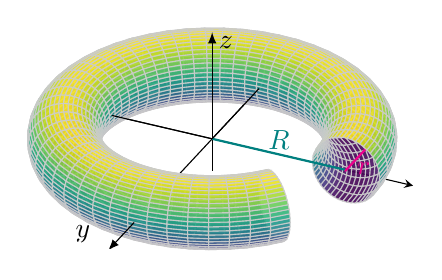
\begin{tikzpicture}
  \begin{axis}[
      axis equal image,
      axis lines=middle,
      xmax=18, zmax=5,
      ticks=none,
      clip bounding box=upper bound,
      % --- 修改部分：更改配色方案 ---
      colormap/viridis, % 使用更现代的 viridis 配色 (也可改为 cool, hot, jet 等)
    ]

    % 绘制环面
    \addplot3[
        domain=0:360,
        y domain=0:320,
        samples=50,
        surf,
        z buffer=sort,
        % --- 修改部分：优化网格线颜色和透明度 ---
        faceted color=black!20, % 让网格线变成浅灰色
        opacity=0.9             % 略微透明，增加立体感
    ]
    ({(12 + 3 * cos(x)) * cos(y)},
     {(12 + 3 * cos(x)) * sin(y)},
     {3 * sin(x)});

    % --- 修改部分：使用坐标轴坐标系绘制半径 R (改为 Teal 色) ---
    \draw [thick, teal] (axis cs: 0,0,0) -- (axis cs: 12,0,0) 
        node [midway, above=-2] {$R$};

    % --- 修改部分：使用坐标轴坐标系绘制半径 r (改为 Magenta 色) ---
    \draw [thick, magenta] (axis cs: 12,-0.2,0) -- (axis cs: 12,3.7,0) 
        node [midway, below right=-3] {$r$};

    % 绘制伪 x, y, z 轴
    \draw [-latex] (axis cs: 0,0,0) -- node [pos=0.9, xshift=0.5em]{$z$}(axis cs: 0,0,10);
    \draw [-latex] (axis cs: 0,-15,0) -- node [pos=0.9, xshift=-1em, yshift=0.5em]{$y$}(axis cs: 0,-20,0);
    
    % 辅助轴线
    \draw (axis cs: 0,0,0) -- (axis cs: 0,9,0);
    \draw (axis cs: 0,0,0) -- (axis cs: -9,0,0);

  \end{axis}
\end{tikzpicture}
\end{document}